% GitLab CI/CD Architecture for Global Workflow
% LaTeX Beamer Presentation
% 
% Compile with: pdflatex gitlab-ci-architecture.tex (run twice for TOC)

\documentclass[aspectratio=169]{beamer}

% Theme and styling
\usetheme{Madrid}
\usecolortheme{whale}
\setbeamertemplate{navigation symbols}{}
\setbeamertemplate{footline}[frame number]

% Packages
\usepackage{graphicx}
\usepackage{tikz}
\usetikzlibrary{shapes,arrows,positioning,fit,backgrounds,calc,decorations.pathreplacing,shadows}
\usepackage{listings}
\usepackage{xcolor}
\usepackage{hyperref}
\usepackage{textcomp}

% Custom colors for a professional look
\definecolor{noaablue}{RGB}{0,51,102}
\definecolor{noaagold}{RGB}{204,153,0}
\definecolor{codegreen}{RGB}{0,128,0}
\definecolor{codegray}{RGB}{128,128,128}
\definecolor{codeblue}{RGB}{0,0,180}
\definecolor{codebg}{RGB}{248,248,248}
\definecolor{codeborder}{RGB}{200,200,200}

% Customize beamer colors
\setbeamercolor{title}{fg=noaablue}
\setbeamercolor{frametitle}{fg=noaablue}
\setbeamercolor{structure}{fg=noaablue}

% Listings configuration - CRITICAL: use literate for hash symbol
\lstset{
  basicstyle=\ttfamily\scriptsize,
  breaklines=true,
  frame=single,
  backgroundcolor=\color{codebg},
  rulecolor=\color{codeborder},
  keywordstyle=\color{codeblue}\bfseries,
  commentstyle=\color{codegray}\itshape,
  stringstyle=\color{codegreen},
  showstringspaces=false,
  tabsize=2,
  xleftmargin=0.5em,
  framexleftmargin=0.5em,
  literate={`}{\textasciigrave}1 {~}{\textasciitilde}1,
  upquote=true,
}

% YAML language definition without comment handling (we'll add comments as text)
\lstdefinelanguage{yaml}{
  keywords={true,false,null,y,n},
  keywordstyle=\color{codegreen},
  basicstyle=\ttfamily\scriptsize,
  sensitive=false,
  stringstyle=\color{codegreen}\ttfamily,
  morestring=[b]',
  morestring=[b]",
  showstringspaces=false,
  breaklines=true,
  frame=single,
  backgroundcolor=\color{codebg},
}

% Title information
\title[GitLab CI for Global Workflow]{GitLab CI/CD Architecture\\for Global Workflow Testing}
\subtitle{Declarative YAML Pipelines, Templates, and Multi-Host Extensibility}
\author{NOAA/EMC Environmental Modeling Center}
\institute{Global Workflow Development Team}
\date{January 2026}

% Logo
\titlegraphic{
  \begin{tikzpicture}[remember picture,overlay]
    \node[opacity=0.15] at (current page.center) {
      \resizebox{8cm}{!}{\textbf{\textsf{NOAA}}}
    };
  \end{tikzpicture}
}

\begin{document}

% =============================================================================
% TITLE SLIDE
% =============================================================================
\begin{frame}
\titlepage
\end{frame}

% =============================================================================
% OUTLINE
% =============================================================================
\begin{frame}[fragile]{Presentation Outline}
\tableofcontents
\end{frame}

% =============================================================================
% SECTION 1: GITLAB PARADIGM
% =============================================================================
\section{The GitLab CI/CD Paradigm}

\begin{frame}[fragile]{GitLab CI/CD: Declarative vs Imperative}

\begin{columns}[T]
\begin{column}{0.48\textwidth}

\begin{block}{\textcolor{noaablue}{Declarative (GitLab YAML)}}
\begin{itemize}
    \item Specify \textbf{what} to do, not \textbf{how}
    \item Configuration as code
    \item Self-documenting pipelines
    \item Reproducible builds
    \item Version controlled alongside code
\end{itemize}
\end{block}

\vspace{0.2cm}
\begin{lstlisting}[language=yaml,basicstyle=\ttfamily\tiny]
build-hera:
  stage: build
  tags: [hera]
  script:
    - make build
\end{lstlisting}
\end{column}

\begin{column}{0.48\textwidth}

\begin{block}{\textcolor{codegray}{Imperative (Traditional Scripts)}}
\begin{itemize}
    \item Step-by-step instructions
    \item External script files
    \item Complex conditionals
    \item Environment-dependent
    \item Harder to maintain
\end{itemize}
\end{block}

\vspace{0.2cm}
\begin{lstlisting}[language=bash,basicstyle=\ttfamily\tiny]
#!/bin/bash
if [ "$MACHINE" = "hera" ]; then
  ssh hera "cd $DIR && make"
fi
\end{lstlisting}
\end{column}
\end{columns}

\vspace{0.3cm}
\begin{center}
\fcolorbox{noaablue}{blue!5}{\parbox{0.88\textwidth}{\centering
\textbf{Key Insight:} GitLab's YAML declaratively defines \textit{what} should happen;\\
the GitLab Runner determines \textit{how} to execute it on each platform.
}}
\end{center}

\end{frame}

% -----------------------------------------------------------------------------
\begin{frame}[fragile]{The Pipeline Configuration File}

\begin{center}
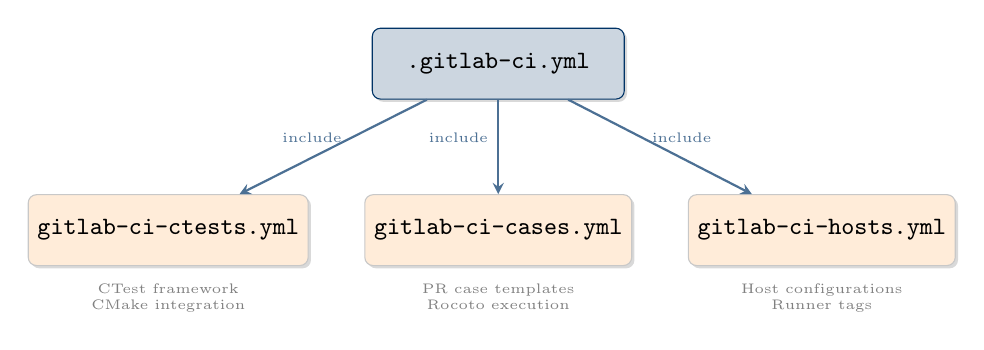
\begin{tikzpicture}[
    node distance=0.8cm,
    file/.style={rectangle, rounded corners=3pt, draw=codeborder, fill=orange!15, 
                 minimum width=3.2cm, minimum height=0.9cm, font=\small\ttfamily,
                 drop shadow={shadow xshift=1pt, shadow yshift=-1pt, opacity=0.3}},
    mainfile/.style={file, fill=noaablue!20, draw=noaablue},
    arrow/.style={->, thick, >=stealth, color=noaablue!70}
]

% Main file
\node[mainfile] (main) {.gitlab-ci.yml};

% Included files
\node[file, below left=1.2cm and 0.8cm of main] (ctests) {gitlab-ci-ctests.yml};
\node[file, below=1.2cm of main] (cases) {gitlab-ci-cases.yml};
\node[file, below right=1.2cm and 0.8cm of main] (hosts) {gitlab-ci-hosts.yml};

% Arrows with labels
\draw[arrow] (main) -- node[left, font=\tiny, pos=0.4] {include} (ctests);
\draw[arrow] (main) -- node[left, font=\tiny, pos=0.4] {include} (cases);
\draw[arrow] (main) -- node[right, font=\tiny, pos=0.4] {include} (hosts);

% Description boxes
\node[below=0.1cm of ctests, font=\tiny, text=codegray, text width=2.8cm, align=center] 
     {CTest framework\\CMake integration};
\node[below=0.1cm of cases, font=\tiny, text=codegray, text width=2.8cm, align=center] 
     {PR case templates\\Rocoto execution};
\node[below=0.1cm of hosts, font=\tiny, text=codegray, text width=2.8cm, align=center] 
     {Host configurations\\Runner tags};

\end{tikzpicture}
\end{center}

\vspace{0.4cm}

\begin{lstlisting}[language=yaml,basicstyle=\ttfamily\scriptsize,title={\small\texttt{.gitlab-ci.yml} -- Include Directive}]
include:
  - local: 'dev/ci/gitlab-ci-ctests.yml'
  - local: 'dev/ci/gitlab-ci-cases.yml'
  - local: 'dev/ci/gitlab-ci-hosts.yml'
\end{lstlisting}

\begin{center}
\textbf{Modular Design:} Split configuration by concern for maintainability
\end{center}

\end{frame}

% =============================================================================
% SECTION 2: STAGES
% =============================================================================
\section{Pipeline Stages}

\begin{frame}[fragile]{Understanding GitLab Stages}

\begin{center}
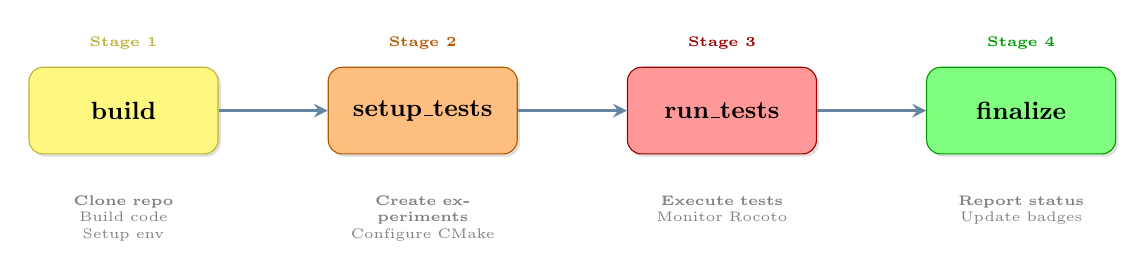
\begin{tikzpicture}[
    stage/.style={rectangle, rounded corners=5pt, draw, minimum width=2.4cm, 
                  minimum height=1.1cm, font=\small\bfseries,
                  drop shadow={shadow xshift=1pt, shadow yshift=-1pt, opacity=0.25}},
    arrow/.style={->, very thick, >=stealth, color=noaablue!60}
]

% Stages with gradient-like fills
\node[stage, fill=yellow!50, draw=yellow!70!black] (build) at (0,0) {build};
\node[stage, fill=orange!50, draw=orange!70!black] (setup) at (3.8,0) {setup\_tests};
\node[stage, fill=red!40, draw=red!60!black] (run) at (7.6,0) {run\_tests};
\node[stage, fill=green!50, draw=green!60!black] (finalize) at (11.4,0) {finalize};

% Arrows
\draw[arrow] (build) -- (setup);
\draw[arrow] (setup) -- (run);
\draw[arrow] (run) -- (finalize);

% Labels below with icons (using text)
\node[below=0.4cm of build, font=\tiny, text width=2.2cm, align=center, text=codegray] 
     {\textbf{Clone repo}\\Build code\\Setup env};
\node[below=0.4cm of setup, font=\tiny, text width=2.2cm, align=center, text=codegray] 
     {\textbf{Create experiments}\\Configure CMake};
\node[below=0.4cm of run, font=\tiny, text width=2.2cm, align=center, text=codegray] 
     {\textbf{Execute tests}\\Monitor Rocoto};
\node[below=0.4cm of finalize, font=\tiny, text width=2.2cm, align=center, text=codegray] 
     {\textbf{Report status}\\Update badges};

% Stage numbers
\node[above=0.1cm of build, font=\tiny\bfseries, text=yellow!70!black] {Stage 1};
\node[above=0.1cm of setup, font=\tiny\bfseries, text=orange!70!black] {Stage 2};
\node[above=0.1cm of run, font=\tiny\bfseries, text=red!60!black] {Stage 3};
\node[above=0.1cm of finalize, font=\tiny\bfseries, text=green!60!black] {Stage 4};

\end{tikzpicture}
\end{center}

\vspace{0.4cm}

\begin{lstlisting}[language=yaml,basicstyle=\ttfamily\scriptsize,title={\small Stage Definition}]
stages:
  - build
  - setup_tests
  - run_tests
  - finalize
\end{lstlisting}

\vspace{0.2cm}
\begin{center}
\fcolorbox{green!50!black}{green!8}{\parbox{0.85\textwidth}{\centering
\textbf{Sequential Execution:} Jobs in stage N must complete before stage N+1 begins\\
\textbf{Parallel Within Stage:} Multiple jobs in same stage run concurrently
}}
\end{center}

\end{frame}

% -----------------------------------------------------------------------------
\begin{frame}[fragile]{Stage Flow: PR Cases vs CTests}

\begin{center}
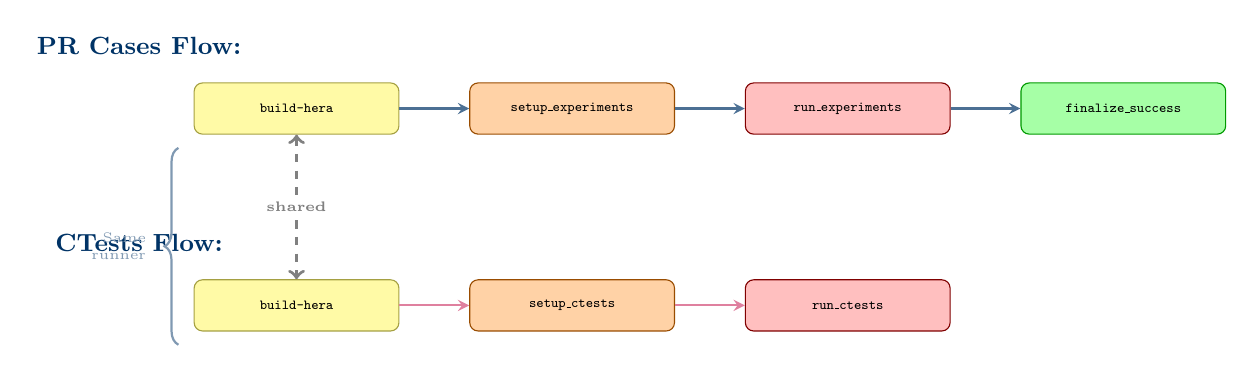
\begin{tikzpicture}[
    node distance=0.6cm,
    box/.style={rectangle, rounded corners=3pt, draw, minimum width=2.6cm, 
                minimum height=0.65cm, font=\tiny\ttfamily},
    arrow/.style={->, thick, >=stealth},
    flowlabel/.style={font=\small\bfseries}
]

% PR Cases flow (top)
\node[flowlabel, color=noaablue] at (-5.5, 1.8) {PR Cases Flow:};

\node[box, fill=yellow!35, draw=yellow!60!black] (pr-build) at (-3.5, 1) {build-hera};
\node[box, fill=orange!35, draw=orange!60!black] (pr-setup) at (0, 1) {setup\_experiments};
\node[box, fill=red!25, draw=red!50!black] (pr-run) at (3.5, 1) {run\_experiments};
\node[box, fill=green!35, draw=green!60!black] (pr-final) at (7, 1) {finalize\_success};

\draw[arrow, color=noaablue!70] (pr-build) -- (pr-setup);
\draw[arrow, color=noaablue!70] (pr-setup) -- (pr-run);
\draw[arrow, color=noaablue!70] (pr-run) -- (pr-final);

% CTests flow (bottom)
\node[flowlabel, color=noaablue] at (-5.5, -0.7) {CTests Flow:};

\node[box, fill=yellow!35, draw=yellow!60!black] (ct-build) at (-3.5, -1.5) {build-hera};
\node[box, fill=orange!35, draw=orange!60!black] (ct-setup) at (0, -1.5) {setup\_ctests};
\node[box, fill=red!25, draw=red!50!black] (ct-run) at (3.5, -1.5) {run\_ctests};

\draw[arrow, color=purple!50] (ct-build) -- (ct-setup);
\draw[arrow, color=purple!50] (ct-setup) -- (ct-run);

% Shared build indicator
\draw[<->, dashed, very thick, color=codegray] (pr-build.south) -- (ct-build.north);
\node[font=\tiny\bfseries, color=codegray, fill=white, inner sep=1pt] at (-3.5, -0.25) {shared};

% Decorative brace for parallel indication
\draw[decorate, decoration={brace, amplitude=5pt, mirror}, thick, color=noaablue!50]
    (-5, 0.5) -- (-5, -2) node[midway, left=8pt, font=\tiny, text width=1.2cm, align=right] 
    {Same\\runner};

\end{tikzpicture}
\end{center}

\vspace{0.3cm}

\begin{lstlisting}[language=yaml,basicstyle=\ttfamily\tiny,title={\small PIPELINE\_TYPE Variable Controls Flow}]
variables:
  PIPELINE_TYPE: pr_cases

rules:
  - if: $PIPELINE_TYPE == "pr_cases" && $CI_PIPELINE_SOURCE == "trigger"
  - if: $PIPELINE_TYPE == "ctests" && $CI_PIPELINE_SOURCE == "trigger"
\end{lstlisting}

\end{frame}

% =============================================================================
% SECTION 3: TEMPLATES
% =============================================================================
\section{Template System}

\begin{frame}[fragile]{YAML Anchors and the \texttt{extends} Keyword}

\begin{columns}[T]
\begin{column}{0.48\textwidth}

\begin{block}{\textcolor{noaablue}{YAML Anchors (\&)}}
Define reusable data blocks
\end{block}

\begin{lstlisting}[language=yaml,basicstyle=\ttfamily\tiny]
.hera_cases_matrix: &hera_cases
  - caseName:
    - "C48_ATM"
    - "C48_S2SW"
    - "C96_atm3DVar"

setup_experiments-hera:
  parallel:
    matrix: *hera_cases
\end{lstlisting}

\vspace{0.2cm}
\fcolorbox{noaablue}{blue!5}{\parbox{0.92\columnwidth}{\tiny
\textbf{Anchors} copy data structures verbatim\\
Use \texttt{\&name} to define, \texttt{*name} to reference
}}
\end{column}

\begin{column}{0.48\textwidth}

\begin{block}{\textcolor{codegreen}{extends Keyword}}
Inherit and override job properties
\end{block}

\begin{lstlisting}[language=yaml,basicstyle=\ttfamily\tiny]
.build_template:
  stage: build
  script:
    - git submodule update
    - dev/ci/scripts/ci_utils.sh build

build-hera:
  extends: .build_template
  variables:
    machine: hera
  tags: [hera]
\end{lstlisting}

\fcolorbox{codegreen}{green!5}{\parbox{0.92\columnwidth}{\tiny
\textbf{extends} merges configs and allows overrides
}}
\end{column}
\end{columns}

\vspace{0.3cm}
\begin{center}
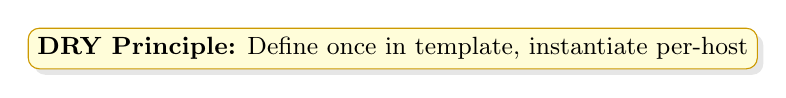
\begin{tikzpicture}
\node[draw=noaagold, rounded corners, fill=yellow!15, font=\small, 
      drop shadow={opacity=0.2}] {
\textbf{DRY Principle:} Define once in template, instantiate per-host
};
\end{tikzpicture}
\end{center}

\end{frame}

% -----------------------------------------------------------------------------
\begin{frame}[fragile]{Template Inheritance Hierarchy}

\begin{center}
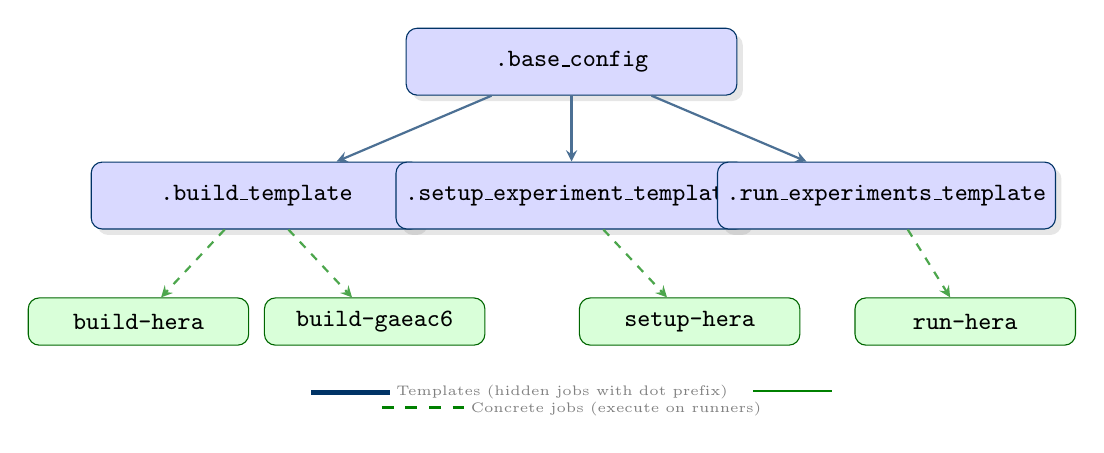
\begin{tikzpicture}[
    node distance=0.8cm,
    template/.style={rectangle, rounded corners=4pt, draw=noaablue, fill=blue!15, 
                     minimum width=4.2cm, minimum height=0.85cm, font=\small\ttfamily,
                     drop shadow={opacity=0.2}},
    job/.style={rectangle, rounded corners=4pt, draw=codegreen!80!black, fill=green!15, 
                minimum width=2.8cm, minimum height=0.6cm, font=\small\ttfamily},
    arrow/.style={->, thick, >=stealth, color=noaablue!70},
    dasharrow/.style={->, dashed, thick, >=stealth, color=codegreen!70}
]

% Base templates (top level)
\node[template] (base) at (0, 3) {.base\_config};

% Second level templates
\node[template] (build) at (-4, 1.3) {.build\_template};
\node[template] (setup) at (0, 1.3) {.setup\_experiment\_template};
\node[template] (run) at (4, 1.3) {.run\_experiments\_template};

% Inheritance arrows from base
\draw[arrow] (base) -- (build);
\draw[arrow] (base) -- (setup);
\draw[arrow] (base) -- (run);

% Concrete jobs (bottom level)
\node[job] (b-hera) at (-5.5, -0.3) {build-hera};
\node[job] (b-gaea) at (-2.5, -0.3) {build-gaeac6};
\node[job] (s-hera) at (1.5, -0.3) {setup-hera};
\node[job] (r-hera) at (5, -0.3) {run-hera};

\draw[dasharrow] (build) -- (b-hera);
\draw[dasharrow] (build) -- (b-gaea);
\draw[dasharrow] (setup) -- (s-hera);
\draw[dasharrow] (run) -- (r-hera);

% Legend
\node[font=\tiny, color=codegray, text width=10cm, align=center] at (0, -1.3) 
     {\textcolor{noaablue}{\rule{1cm}{2pt}} Templates (hidden jobs with dot prefix) \quad 
      \textcolor{codegreen}{\rule[0.5ex]{1cm}{1pt}\hspace{-1cm}\rule[0.5ex]{0.15cm}{1pt}\hspace{0.15cm}\rule[0.5ex]{0.15cm}{1pt}\hspace{0.15cm}\rule[0.5ex]{0.15cm}{1pt}\hspace{0.15cm}\rule[0.5ex]{0.15cm}{1pt}} Concrete jobs (execute on runners)};

\end{tikzpicture}
\end{center}

\vspace{0.2cm}

\begin{lstlisting}[language=yaml,basicstyle=\ttfamily\tiny,title={\small Multiple Inheritance with extends}]
.build_template:
  extends:
    - .base_config
    - .failure_cleanup_template
  stage: build
  script:
    - git submodule update --init --recursive
    - source dev/ush/gw_setup.sh
    - dev/ci/scripts/utils/ci_utils.sh build
\end{lstlisting}

\end{frame}

% -----------------------------------------------------------------------------
\begin{frame}[fragile]{The Base Configuration Template}

\begin{lstlisting}[language=yaml,basicstyle=\ttfamily\tiny,title={\small .base\_config -- Shared by ALL Jobs}]
.base_config:
  variables:
    badge_GIST_ID: "66059582886cb5c2485ff64bf24e7f93"
    GIT_STRATEGY: none
  before_script:
    - |
      echo "Starting GitLab CI pipeline for global-workflow project"
      PR_NUMBER=${PR_NUMBER:-0}
      
      export GW_RUN_PATH="${CI_BUILDS_DIR}/${WORKSPACE_ID}"
      export GW_HOMEgfs="${GIT_CLONE_PATH}"
      export RUNTESTS_DIR="${GW_RUN_PATH}/RUNTESTS"
      
      export GH=$(which gh 2>/dev/null || echo "${HOME}/bin/gh")
      
      if [ ! -d "${GW_HOMEgfs}" ]; then
        echo "ERROR: GW_HOMEgfs directory does not exist"
        exit 1
      fi
\end{lstlisting}

\vspace{0.2cm}
\begin{center}
\fcolorbox{orange!70!black}{orange!10}{\parbox{0.9\textwidth}{\centering
\textbf{before\_script} runs before every job's main script\\
Sets up environment variables, validates paths, configures GitHub CLI
}}
\end{center}

\end{frame}

% =============================================================================
% SECTION 4: MULTI-MODALITY
% =============================================================================
\section{Multi-Modality: PR Cases \& CTests}

\begin{frame}[fragile]{Two Testing Modalities}

\begin{center}
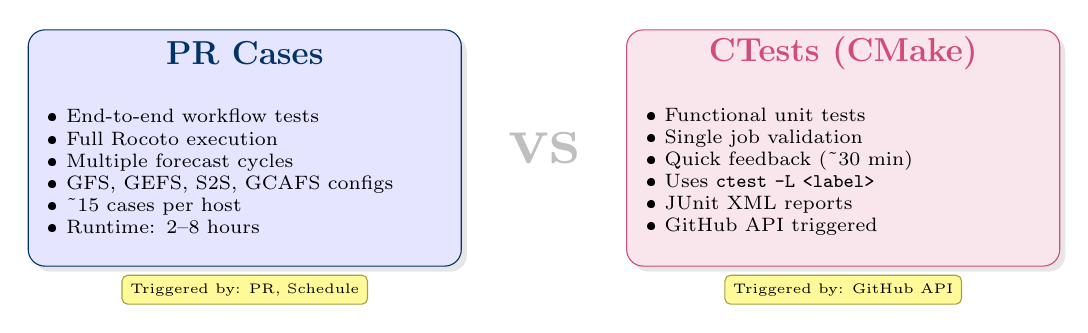
\begin{tikzpicture}[
    box/.style={rectangle, rounded corners=6pt, draw, minimum width=5.5cm, 
                minimum height=3cm, font=\small,
                drop shadow={shadow xshift=2pt, shadow yshift=-2pt, opacity=0.2}},
]

% PR Cases box
\node[box, fill=blue!10, draw=noaablue] (pr) at (-3.8, 0) {};
\node[font=\bfseries\large, color=noaablue] at (-3.8, 1.2) {PR Cases};
\node[font=\scriptsize, text width=5cm, align=left] at (-3.8, -0.3) {
\textbullet\ End-to-end workflow tests\\
\textbullet\ Full Rocoto execution\\
\textbullet\ Multiple forecast cycles\\
\textbullet\ GFS, GEFS, S2S, GCAFS configs\\
\textbullet\ \textasciitilde15 cases per host\\
\textbullet\ Runtime: 2--8 hours
};

% CTests box
\node[box, fill=purple!10, draw=purple!70] (ct) at (3.8, 0) {};
\node[font=\bfseries\large, color=purple!70] at (3.8, 1.2) {CTests (CMake)};
\node[font=\scriptsize, text width=5cm, align=left] at (3.8, -0.3) {
\textbullet\ Functional unit tests\\
\textbullet\ Single job validation\\
\textbullet\ Quick feedback (\textasciitilde30 min)\\
\textbullet\ Uses \texttt{ctest -L <label>}\\
\textbullet\ JUnit XML reports\\
\textbullet\ GitHub API triggered
};

% Trigger badges
\node[font=\tiny, fill=yellow!40, rounded corners=2pt, draw=yellow!60!black, 
      inner sep=3pt] at (-3.8, -1.8) {Triggered by: PR, Schedule};
\node[font=\tiny, fill=yellow!40, rounded corners=2pt, draw=yellow!60!black, 
      inner sep=3pt] at (3.8, -1.8) {Triggered by: GitHub API};

% VS indicator
\node[font=\Huge\bfseries, color=codegray!50] at (0, 0) {vs};

\end{tikzpicture}
\end{center}

\vspace{0.2cm}

\begin{lstlisting}[language=yaml,basicstyle=\ttfamily\tiny,title={\small PIPELINE\_TYPE Variable Switches Modality}]
variables:
  PIPELINE_TYPE: pr_cases
\end{lstlisting}

\end{frame}

% -----------------------------------------------------------------------------
\begin{frame}[fragile]{CTest Framework Configuration}

\begin{lstlisting}[language=yaml,basicstyle=\ttfamily\tiny,title={\small gitlab-ci-ctests.yml -- CTest Templates}]
.setup_ctests_template:
  extends:
    - .base_config
    - .failure_cleanup_template
  stage: setup_tests
  script: |
    source "${GW_HOMEgfs}/dev/ush/gw_setup.sh"
    cd "${GW_HOMEgfs}/dev/ctests"
    mkdir -p build && cd build
    cmake -S "${GW_HOMEgfs}"
    ctest -N

.run_ctests_template:
  stage: run_tests
  script: |
    cd "${GW_HOMEgfs}/dev/ctests/build"
    ctest -L "${CTEST_NAME}" --output-junit result.xml --stop-on-failure
  artifacts:
    reports:
      junit: ${GIT_CLONE_PATH}/dev/ctests/build/result.xml
\end{lstlisting}

\vspace{0.2cm}
\begin{center}
\fcolorbox{purple!70}{purple!8}{\parbox{0.9\textwidth}{\centering
CTests use CMake's testing framework with JUnit XML output\\
GitLab automatically parses JUnit for test result visualization
}}
\end{center}

\end{frame}

% -----------------------------------------------------------------------------
\begin{frame}[fragile]{CTest Matrix: Parallel Test Execution}

\begin{lstlisting}[language=yaml,basicstyle=\ttfamily\tiny,title={\small CTest Label Matrix -- Each Runs as Separate Job}]
.ctests_cases_template:
  extends: .run_ctests_template
  parallel:
    matrix:
      - CTEST_NAME:
        - C48_ATM-gfs_stage_ic
        - C48_ATM-gfs_fcst_seg0
        - C48_ATM-gfs_atmos_prod_f000-f002
        - C48_ATM-gfs_tracker
        - C48_ATM-gfs_genesis
        - C48_S2SW-gfs_fcst_seg0
        - C48_S2SW-gfs_ocean_prod_f006
        - C48_S2SW-gfs_ice_prod_f006
        - C48_S2SWA_gefs-gefs_fcst_mem001_seg0
\end{lstlisting}

\vspace{0.3cm}
\begin{center}
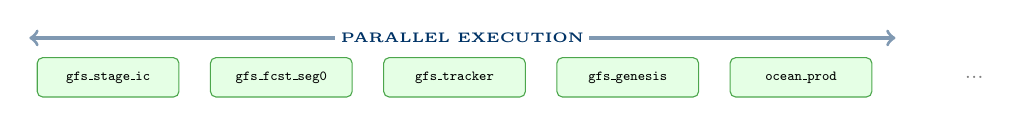
\begin{tikzpicture}[
    testbox/.style={rectangle, rounded corners=2pt, draw=codegreen!70, fill=green!10,
                    minimum width=1.8cm, minimum height=0.5cm, font=\tiny\ttfamily}
]
% Show parallel execution
\node[testbox] at (0, 0) {gfs\_stage\_ic};
\node[testbox] at (2.2, 0) {gfs\_fcst\_seg0};
\node[testbox] at (4.4, 0) {gfs\_tracker};
\node[testbox] at (6.6, 0) {gfs\_genesis};
\node[testbox] at (8.8, 0) {ocean\_prod};

\node[font=\scriptsize, color=codegray] at (11, 0) {...};

% Arrow indicating parallel
\draw[<->, very thick, color=noaablue!50] (-1, 0.5) -- (10, 0.5);
\node[font=\tiny\bfseries, color=noaablue, fill=white, inner sep=2pt] at (4.5, 0.5) 
     {PARALLEL EXECUTION};
\end{tikzpicture}
\end{center}

\begin{center}
\textbf{9 CTests run in parallel} across available runners
\end{center}

\end{frame}

% =============================================================================
% SECTION 5: HOST EXTENSIBILITY
% =============================================================================
\section{Host-Specific Extensibility}

\begin{frame}[fragile]{The Host Configuration File}

\begin{center}
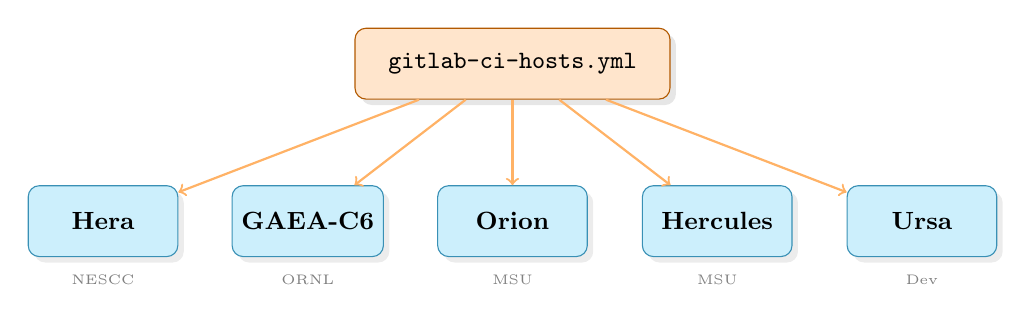
\begin{tikzpicture}[
    host/.style={rectangle, rounded corners=4pt, draw=cyan!70!black, fill=cyan!20, 
                 minimum width=1.9cm, minimum height=0.9cm, font=\small\bfseries,
                 drop shadow={opacity=0.15}},
]

% Host nodes
\node[host] (hera) at (0, 0) {Hera};
\node[host] (gaea) at (2.6, 0) {GAEA-C6};
\node[host] (orion) at (5.2, 0) {Orion};
\node[host] (herc) at (7.8, 0) {Hercules};
\node[host] (ursa) at (10.4, 0) {Ursa};

% Central file
\node[draw=orange!70!black, fill=orange!20, rounded corners=4pt, font=\small\ttfamily,
      minimum width=4cm, minimum height=0.9cm,
      drop shadow={opacity=0.2}] (file) at (5.2, 2) {gitlab-ci-hosts.yml};

% Connections
\foreach \h in {hera, gaea, orion, herc, ursa} {
    \draw[->, thick, color=orange!60] (file) -- (\h);
}

% HPC icons (text-based)
\node[below=0.1cm of hera, font=\tiny, color=codegray] {NESCC};
\node[below=0.1cm of gaea, font=\tiny, color=codegray] {ORNL};
\node[below=0.1cm of orion, font=\tiny, color=codegray] {MSU};
\node[below=0.1cm of herc, font=\tiny, color=codegray] {MSU};
\node[below=0.1cm of ursa, font=\tiny, color=codegray] {Dev};

\end{tikzpicture}
\end{center}

\vspace{0.3cm}

\begin{lstlisting}[language=yaml,basicstyle=\ttfamily\tiny,title={\small Host-Specific Case Matrices (YAML Anchors)}]
.hera_cases_matrix: &hera_cases
  - caseName: ["C48_ATM", "C48_S2SW", "C48_S2SWA_gefs", "C48mx500_3DVarAOWCDA",
               "C96C48_hybatmDA", "C96C48_hybatmsnowDA", "C96_atm3DVar", ...]

.gaeac6_cases_matrix: &gaeac6_cases
  - caseName: ["C48_ATM", "C48_S2SW", "C96_atm3DVar", ...]

.orion_cases_matrix: &orion_cases
  - caseName: ["C48_ATM", "C48_S2SW", "C96_atm3DVar", ...]
\end{lstlisting}

\begin{center}
\fcolorbox{cyan!70!black}{cyan!8}{\parbox{0.85\textwidth}{\centering
Each HPC platform runs a \textbf{different subset of tests}\\
based on available resources, software, and queue policies
}}
\end{center}

\end{frame}

% -----------------------------------------------------------------------------
\begin{frame}[fragile]{Host Job Instantiation Pattern}

\begin{lstlisting}[language=yaml,basicstyle=\ttfamily\tiny,title={\small Concrete Jobs Inherit Templates + Host-Specific Config}]
setup_experiments-hera:
  extends: .setup_experiment_template
  variables:
    machine: hera
  tags:
    - hera
  parallel:
    matrix: *hera_cases
  needs:
    - build-hera
  rules:
    - if: $PIPELINE_TYPE == "pr_cases" && 
          ($CI_PIPELINE_SOURCE == "trigger" || $CI_PIPELINE_SOURCE == "schedule") &&
          ($RUN_ON_MACHINES =~ /\bhera\b|all/)

run_experiments-hera:
  extends: .run_experiments_template
  variables:
    machine: hera
  tags: [hera]
  parallel:
    matrix: *hera_cases
  needs: [setup_experiments-hera]
\end{lstlisting}

\end{frame}

% -----------------------------------------------------------------------------
\begin{frame}[fragile]{Adding a New Host: The Pattern}

\begin{center}
\fcolorbox{noaagold}{yellow!15}{\parbox{0.95\textwidth}{
\centering\textbf{To add a new HPC platform (e.g., ``jet''):}
}}
\end{center}

\vspace{0.2cm}

\begin{columns}[T]
\begin{column}{0.48\textwidth}
\begin{lstlisting}[language=yaml,basicstyle=\ttfamily\tiny,title={\small Step 1: Define case matrix}]
.jet_cases_matrix: &jet_cases
  - caseName:
    - "C48_ATM"
    - "C48_S2SW"
\end{lstlisting}

\begin{lstlisting}[language=yaml,basicstyle=\ttfamily\tiny,title={\small Step 2: Add build job}]
build-jet:
  extends: .build_template
  variables:
    machine: jet
  tags: [jet]
  rules:
    - if: $RUN_ON_MACHINES =~ /jet|all/
\end{lstlisting}
\end{column}

\begin{column}{0.48\textwidth}
\begin{lstlisting}[language=yaml,basicstyle=\ttfamily\tiny,title={\small Step 3: Add setup/run jobs}]
setup_experiments-jet:
  extends: .setup_experiment_template
  variables:
    machine: jet
  tags: [jet]
  parallel:
    matrix: *jet_cases
  needs: [build-jet]

run_experiments-jet:
  extends: .run_experiments_template
  variables:
    machine: jet
  tags: [jet]
  parallel:
    matrix: *jet_cases
  needs: [setup_experiments-jet]
\end{lstlisting}
\end{column}
\end{columns}

\vspace{0.2cm}
\begin{center}
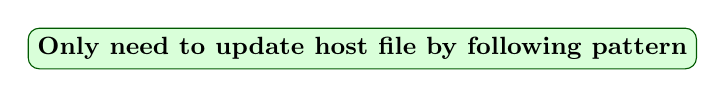
\begin{tikzpicture}
\node[draw=codegreen!70!black, rounded corners, fill=green!15, font=\small] {
\textbf{Only need to update host file by following pattern}
};
\end{tikzpicture}
\end{center}

\end{frame}

% -----------------------------------------------------------------------------
\begin{frame}[fragile]{Runner Tags and Job Routing}

\begin{center}
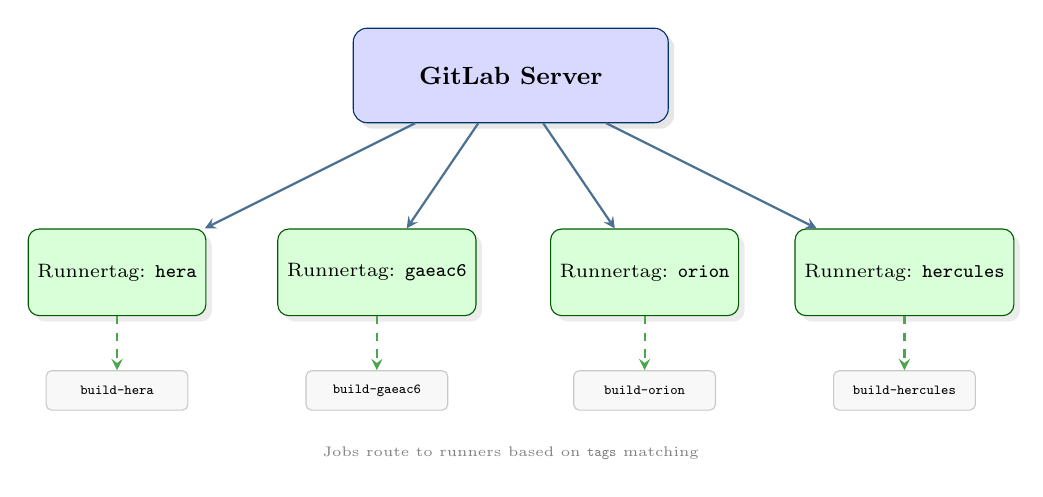
\begin{tikzpicture}[
    node distance=1cm,
    runner/.style={rectangle, rounded corners=4pt, draw=codegreen!70!black, fill=green!15, 
                   minimum width=2.2cm, minimum height=1.1cm, font=\scriptsize,
                   drop shadow={opacity=0.15}},
    job/.style={rectangle, rounded corners=2pt, draw=codeborder, fill=codebg, 
                minimum width=1.8cm, minimum height=0.5cm, font=\tiny\ttfamily},
    arrow/.style={->, thick, >=stealth}
]

% GitLab Server
\node[draw=noaablue, fill=blue!15, rounded corners=5pt, 
      minimum width=4cm, minimum height=1.2cm, font=\small\bfseries,
      drop shadow={opacity=0.2}] (gitlab) at (0, 2.5) {GitLab Server};

% Runners
\node[runner] (hera-r) at (-5, 0) {Runner\\tag: \texttt{hera}};
\node[runner] (gaea-r) at (-1.7, 0) {Runner\\tag: \texttt{gaeac6}};
\node[runner] (orion-r) at (1.7, 0) {Runner\\tag: \texttt{orion}};
\node[runner] (herc-r) at (5, 0) {Runner\\tag: \texttt{hercules}};

% Jobs
\node[job] (j1) at (-5, -1.5) {build-hera};
\node[job] (j2) at (-1.7, -1.5) {build-gaeac6};
\node[job] (j3) at (1.7, -1.5) {build-orion};
\node[job] (j4) at (5, -1.5) {build-hercules};

% Arrows from GitLab to runners
\draw[arrow, color=noaablue!70] (gitlab) -- (hera-r);
\draw[arrow, color=noaablue!70] (gitlab) -- (gaea-r);
\draw[arrow, color=noaablue!70] (gitlab) -- (orion-r);
\draw[arrow, color=noaablue!70] (gitlab) -- (herc-r);

% Arrows from runners to jobs
\draw[arrow, dashed, color=codegreen!70] (hera-r) -- (j1);
\draw[arrow, dashed, color=codegreen!70] (gaea-r) -- (j2);
\draw[arrow, dashed, color=codegreen!70] (orion-r) -- (j3);
\draw[arrow, dashed, color=codegreen!70] (herc-r) -- (j4);

% Decorative cloud for "distributed"
\node[font=\tiny, color=codegray] at (0, -2.3) 
     {Jobs route to runners based on \texttt{tags} matching};

\end{tikzpicture}
\end{center}

\begin{lstlisting}[language=yaml,basicstyle=\ttfamily\tiny,title={\small Tags Route Jobs to Correct Runner}]
build-hera:
  tags:
    - hera
\end{lstlisting}

\end{frame}

% =============================================================================
% SECTION 6: RULES AND CONDITIONALS
% =============================================================================
\section{Conditional Execution}

\begin{frame}[fragile]{Rules: Controlling When Jobs Run}

\begin{lstlisting}[language=yaml,basicstyle=\ttfamily\scriptsize,title={\small Rule Example}]
rules:
  - if: $PIPELINE_TYPE == "pr_cases" &&
        ($CI_PIPELINE_SOURCE == "trigger" ||
         $CI_PIPELINE_SOURCE == "schedule") &&
        ($RUN_ON_MACHINES =~ /\bhera\b|all/)
\end{lstlisting}

\vspace{0.4cm}

\begin{center}
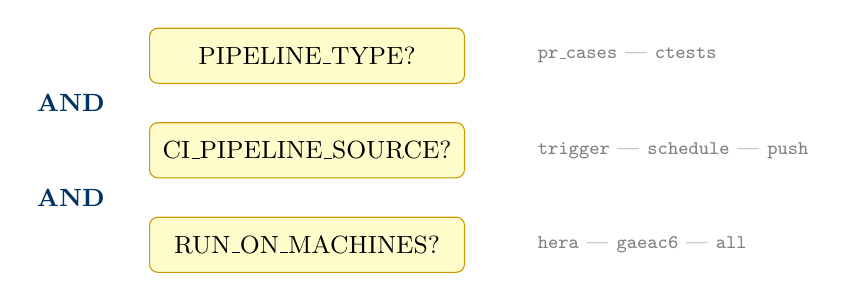
\begin{tikzpicture}[
    cond/.style={rectangle, rounded corners=3pt, draw=noaagold, fill=yellow!20, 
                 minimum width=4cm, minimum height=0.7cm, font=\small},
    arrow/.style={->, thick, color=noaablue!60}
]

\node[cond] (type) at (0, 2) {PIPELINE\_TYPE?};
\node[cond] (source) at (0, 0.8) {CI\_PIPELINE\_SOURCE?};
\node[cond] (machine) at (0, -0.4) {RUN\_ON\_MACHINES?};

\node[font=\scriptsize, right=0.8cm of type, text=codegray] {\texttt{pr\_cases} | \texttt{ctests}};
\node[font=\scriptsize, right=0.8cm of source, text=codegray] {\texttt{trigger} | \texttt{schedule} | \texttt{push}};
\node[font=\scriptsize, right=0.8cm of machine, text=codegray] {\texttt{hera} | \texttt{gaeac6} | \texttt{all}};

% Logical AND indicators
\node[font=\small\bfseries, color=noaablue] at (-3, 1.4) {AND};
\node[font=\small\bfseries, color=noaablue] at (-3, 0.2) {AND};

\end{tikzpicture}
\end{center}

\vspace{0.3cm}

\begin{center}
\fcolorbox{red!60!black}{red!8}{\parbox{0.9\textwidth}{\centering
\textbf{Rules prevent accidental runs:} Jobs only execute when\\
triggered correctly, not on merge to develop or manual push
}}
\end{center}

\end{frame}

% =============================================================================
% SECTION 7: ERROR HANDLING
% =============================================================================
\section{Error Handling \& Reporting}

\begin{frame}[fragile]{Failure Cleanup Template}

\begin{lstlisting}[language=yaml,basicstyle=\ttfamily\tiny,title={\small .failure\_cleanup\_template -- after\_script}]
.failure_cleanup_template:
  after_script:
    - |
      if [[ ${CI_JOB_STATUS} == "failed" ]]; then
        Machine="${machine^}"
        
        if [[ "${GFS_CI_RUN_TYPE}" == "pr_cases" && "${PR_NUMBER}" != 0 ]]; then
          ${GH} pr edit ${PR_NUMBER} --repo ${GW_REPO_URL} \
            --add-label "CI-${Machine}-Failed" \
            --remove-label "CI-${Machine}-Building" \
            --remove-label "CI-${Machine}-Running"
            
          comment_body="**BUILD FAILED** on ${Machine}..."
          ${GH} pr comment ${PR_NUMBER} --body "${comment_body}"
          
        elif [[ "${GFS_CI_RUN_TYPE}" == "nightly" ]]; then
          curl "https://img.shields.io/badge/${machine}_nightly-failed-red" \
            -o badge.svg
          ${GH} gist edit "${badge_GIST_ID}" --add badge.svg
        fi
      fi
\end{lstlisting}

\end{frame}

% -----------------------------------------------------------------------------
\begin{frame}[fragile]{GitHub Integration: Labels \& Badges}

\begin{center}
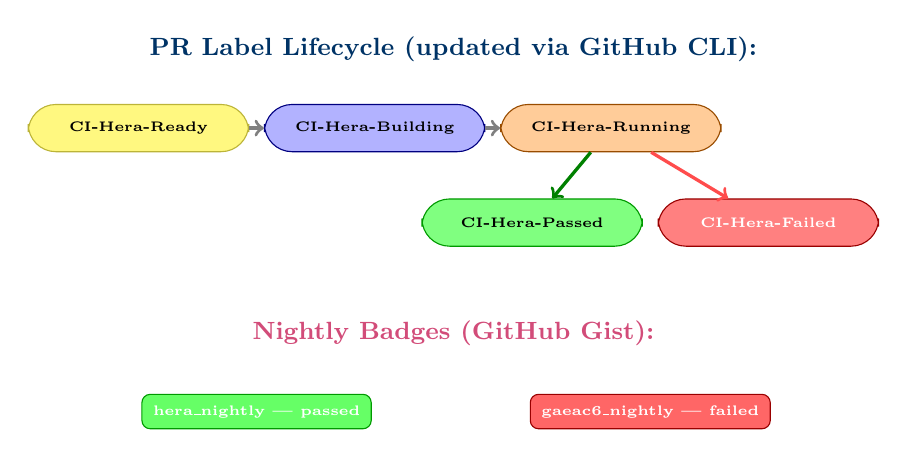
\begin{tikzpicture}[
    node distance=0.5cm,
    label/.style={rectangle, rounded corners=10pt, draw, minimum width=2.8cm, 
                  minimum height=0.6cm, font=\tiny\bfseries},
]

% PR Lifecycle labels
\node[font=\small\bfseries, color=noaablue] at (0, 2.8) {PR Label Lifecycle (updated via GitHub CLI):};

\node[label, fill=yellow!50, draw=yellow!70!black] (ready) at (-4, 1.8) {CI-Hera-Ready};
\node[label, fill=blue!30, draw=blue!50!black] (building) at (-1, 1.8) {CI-Hera-Building};
\node[label, fill=orange!40, draw=orange!60!black] (running) at (2, 1.8) {CI-Hera-Running};
\node[label, fill=green!50, draw=green!60!black] (passed) at (1, 0.6) {CI-Hera-Passed};
\node[label, fill=red!50, draw=red!60!black, text=white] (failed) at (4, 0.6) {CI-Hera-Failed};

\draw[->, very thick, color=codegray] (ready) -- (building);
\draw[->, very thick, color=codegray] (building) -- (running);
\draw[->, very thick, color=codegreen] (running) -- (passed);
\draw[->, very thick, color=red!70] (running) -- (failed);

% Badge examples
\node[font=\small\bfseries, color=purple!70] at (0, -0.8) {Nightly Badges (GitHub Gist):};

\node[draw=green!60!black, fill=green!60, rounded corners=3pt, font=\tiny\bfseries, 
      inner sep=4pt, text=white] at (-2.5, -1.8) {hera\_nightly | passed};
\node[draw=red!60!black, fill=red!60, rounded corners=3pt, font=\tiny\bfseries, 
      inner sep=4pt, text=white] at (2.5, -1.8) {gaeac6\_nightly | failed};

\end{tikzpicture}
\end{center}

\vspace{0.3cm}

\begin{center}
\fcolorbox{noaablue}{blue!8}{\parbox{0.9\textwidth}{\centering
\textbf{Bidirectional Integration:}\\
GitHub triggers GitLab $\rightarrow$ GitLab updates GitHub labels/comments/badges
}}
\end{center}

\end{frame}

% =============================================================================
% SECTION 8: SUMMARY
% =============================================================================
\section{Summary}

\begin{frame}[fragile]{Architecture Summary}

\begin{center}
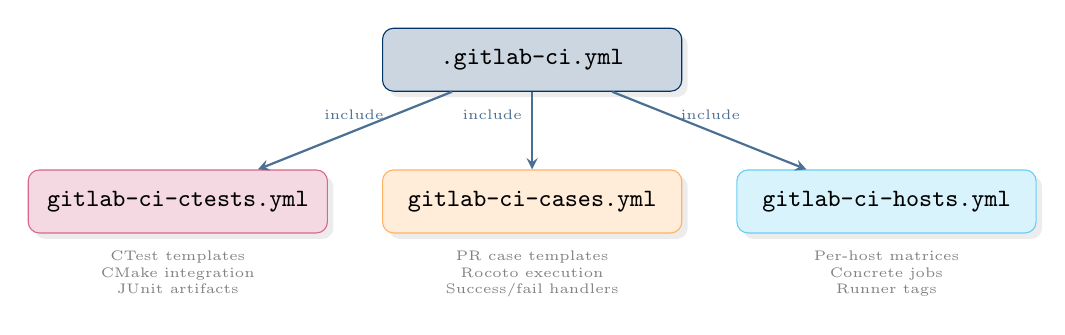
\begin{tikzpicture}[
    node distance=0.8cm,
    file/.style={rectangle, rounded corners=4pt, draw, minimum width=3.8cm, 
                 minimum height=0.8cm, font=\small\ttfamily,
                 drop shadow={opacity=0.15}},
    arrow/.style={->, thick, >=stealth, color=noaablue!70}
]

% Files
\node[file, fill=noaablue!20, draw=noaablue] (main) at (0, 3) {.gitlab-ci.yml};
\node[file, fill=purple!15, draw=purple!60] (ctests) at (-4.5, 1.2) {gitlab-ci-ctests.yml};
\node[file, fill=orange!15, draw=orange!60] (cases) at (0, 1.2) {gitlab-ci-cases.yml};
\node[file, fill=cyan!15, draw=cyan!60] (hosts) at (4.5, 1.2) {gitlab-ci-hosts.yml};

% Arrows
\draw[arrow] (main) -- node[left, font=\tiny, pos=0.3] {include} (ctests);
\draw[arrow] (main) -- node[left, font=\tiny, pos=0.3] {include} (cases);
\draw[arrow] (main) -- node[right, font=\tiny, pos=0.3] {include} (hosts);

% Contents
\node[font=\tiny, below=0.1cm of ctests, text width=3.2cm, align=center, color=codegray] {
CTest templates\\CMake integration\\JUnit artifacts
};

\node[font=\tiny, below=0.1cm of cases, text width=3.2cm, align=center, color=codegray] {
PR case templates\\Rocoto execution\\Success/fail handlers
};

\node[font=\tiny, below=0.1cm of hosts, text width=3.2cm, align=center, color=codegray] {
Per-host matrices\\Concrete jobs\\Runner tags
};

\end{tikzpicture}
\end{center}

\vspace{0.2cm}

\begin{columns}[T]
\begin{column}{0.48\textwidth}
\begin{block}{\textcolor{noaablue}{Key Design Principles}}
\begin{itemize}
    \item Declarative YAML configuration
    \item DRY via templates and anchors
    \item Separation of concerns
    \item Easy host extensibility
\end{itemize}
\end{block}
\end{column}
\begin{column}{0.48\textwidth}
\begin{block}{\textcolor{codegreen}{Benefits Achieved}}
\begin{itemize}
    \item 5 HPC platforms supported
    \item 2 testing modalities (PR/CTest)
    \item Automated GitHub integration
    \item \textasciitilde50 lines to add new host
\end{itemize}
\end{block}
\end{column}
\end{columns}

\end{frame}

% -----------------------------------------------------------------------------
\begin{frame}[fragile]{Quick Reference: Key YAML Constructs}

\begin{center}
\small
\begin{tabular}{|>{\ttfamily\scriptsize}l|>{\ttfamily\scriptsize}l|p{5.5cm}|}
\hline
\textbf{\textrm{Construct}} & \textbf{\textrm{Syntax}} & \textbf{\textrm{\scriptsize Purpose}} \\
\hline
Hidden job & .template\_name: & Define reusable template (not executed) \\
\hline
Extends & extends: .template & Inherit from template(s) \\
\hline
Anchor & \&name & Define reusable data block \\
\hline
Alias & *name & Reference anchor data \\
\hline
Include & include: - local: & Import from other YAML files \\
\hline
Parallel matrix & parallel: matrix: & Generate multiple jobs from list \\
\hline
Tags & tags: [host] & Route job to specific runner \\
\hline
Rules & rules: - if: & Conditional job execution \\
\hline
Needs & needs: [job] & Explicit job dependency \\
\hline
Artifacts & artifacts: reports: & Collect test results \\
\hline
\end{tabular}
\end{center}

\end{frame}

% -----------------------------------------------------------------------------
\begin{frame}[fragile]{Questions?}

\begin{center}
\vspace{0.5cm}


\begin{tikzpicture}
\node[font=\Huge\bfseries, color=noaablue!30] {?};
\end{tikzpicture}

\vspace{0.5cm}

{\Large\bfseries Thank you!}

\vspace{0.5cm}

\begin{tabular}{rl}
\textbf{GitHub:} & \url{github.com/NOAA-EMC/global-workflow} \\
\textbf{GitLab:} & GitLab vLab (internal) \\
\textbf{CI Docs:} & \texttt{dev/ci/} directory \\
\end{tabular}

\vspace{0.8cm}

\fcolorbox{codeborder}{codebg}{\parbox{0.7\textwidth}{\centering
\small Global Workflow CI/CD Architecture\\
\textbf{NOAA/EMC Environmental Modeling Center}
}}

\end{center}

\end{frame}

\end{document}
